
\chapter{Fonctionnement de notre système}
\label{chap:fonctionnement}

Suite à notre état de l'art et analyse fonctionnelle, nous avons imaginé un système s'appuyant des radiogoniomètres à effet Doppler et plus particulièrement sur le Montréal 3v2.


\section{Principe}

Nous avons imaginé positionner plusieurs radiogoniomètre à effet Doppler équivalent au Montréal 3v2. Ainsi chaque appareil indiquerai la direction du drone par rapport à sa position. Chacun d'eux serai connecter à un ordinateur centrale qui analyserai chacune des positions données par les radiogoniomètres et en déduirait la position du drone dans l'espace.

~\\

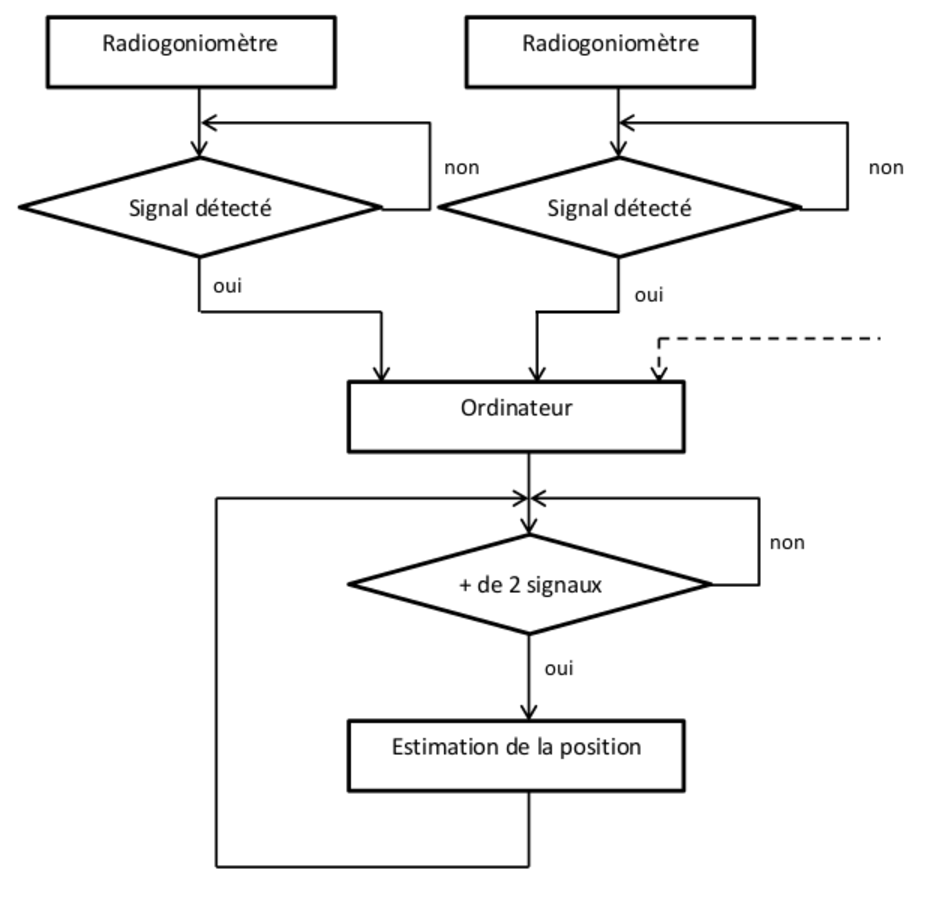
\includegraphics[width=0.8\textwidth]{SMART_logic}
\captionof{figure}{Schéma Logique du système}







%%% Local Variables: 
%%% mode: latex
%%% TeX-master: "rapport_analyse"
%%% End: 
